\documentclass[11pt]{article}
\usepackage[utf8]{inputenc}
\usepackage[T1]{fontenc}
\usepackage{amsmath}
\usepackage{amssymb} % Needed for \eth
\usepackage{graphicx}
\usepackage{geometry}
\usepackage{tikz}
\usepackage{ulem} 
\usepackage{pgfplots}
\pgfplotsset{compat=1.18}
\usepackage{tikz}
\usetikzlibrary{patterns}% For underline, using normalem to avoid messing with \emph

\geometry{a4paper, margin=1in}
\usetikzlibrary{positioning, arrows.meta, shapes.geometric, calc} % For TikZ diagrams

% Custom commands (optional)
\newcommand{\avg}[1]{\overline{#1}}
\newcommand{\prob}[1]{P(#1)}
\newcommand{\ProbDens}[1]{\mathcal{P}(#1)} % Using script P for density
\newcommand{\vect}[1]{\vec{#1}}
\newcommand{\dd}[1]{\mathrm{d}#1} % Differential d
\newcommand{\pderiv}[2]{\frac{\partial #1}{\partial #2}}
\newcommand{\deriv}[2]{\frac{\mathrm{d} #1}{\mathrm{d} #2}}
\newcommand{\muState}{\mu\text{-state}} % Microstate
\newcommand{\OmegaE}{\Omega(E)}
\newcommand{\omegaE}{\omega(E)}
\newcommand{\PhiE}{\Phi(E)}
\newcommand{\deltaE}{\delta E}
\newcommand{\ethbar}{\text{\it{đ}}} % \eth symbol for inexact differential

\title{Physics 415 - Lecture 6}
\date{February 3, 2025}
\author{} % Author not specified

\begin{document}

\maketitle
\thispagestyle{empty}

\section*{Summary}

\begin{itemize}
    \item Macrostate of a system specified by:
    \begin{itemize}
        \item Fixed external parameters $(x_1, x_2, \dots, x_n)$. Ex: $x=V=$ Volume.
        \item Additional conditions on the system. Ex: Energy $E = \text{const}$ (closed system).
    \end{itemize}
    \item Interaction between macroscopic systems A and B (really, ensembles):
    \begin{itemize}
        \item Interaction leads to change in mean energy $\avg{E}$ of A (say).
        \item Interaction types:
        \begin{itemize}
            \item Thermal (Heat exchange $Q$).
            \item Mechanical (Work $W$).
        \end{itemize}
        \item First Law of Thermodynamics (infinitesimal form):
        \[ \ethbar Q = d\avg{E} + \ethbar W \]
        where $d\avg{E}$ = small change in mean energy, $\ethbar Q$ = small heat absorbed by A, $\ethbar W$ = small work done *by* A.
    \end{itemize}
\end{itemize}

\section*{Exact and Inexact Differentials (Mathematical Aside)}

Explain difference between "$d$" and "$\ethbar$".

Consider a function $F(x,y)$ of two variables $x$ and $y$. A small change $x \to x+dx$, $y \to y+dy$ leads to $F(x,y) \to F(x+dx, y+dy)$. The change $dF$ is:
\[ dF = F(x+dx, y+dy) - F(x,y) \]
Using Taylor expansion for small $dx, dy$:
\[ dF = \pderiv{F}{x} dx + \pderiv{F}{y} dy \]
Let $A(x,y) = \pderiv{F}{x}$ and $B(x,y) = \pderiv{F}{y}$. Then $dF = A(x,y)dx + B(x,y)dy$.
This is called an "exact differential". It is the differential of an actual function $F(x,y)$.

\begin{itemize}
    \item In going from an initial point $(x_i, y_i)$ to a final point $(x_f, y_f)$, the net change in $F$ is:
    \[ \Delta F = F(x_f, y_f) - F(x_i, y_i) = \int_i^f dF = \int_i^f (A dx + B dy) \]
    \item The integral $\int_i^f dF$ is independent of the path taken in the $(x,y)$-plane between $(x_i, y_i)$ and $(x_f, y_f)$. $F$ is a "state function".
\end{itemize}

Now consider infinitesimal quantities of the form $\tilde{A}(x,y)dx + \tilde{B}(x,y)dy$ that are *not* the differential of any function $G(x,y)$. That is, there is no function $G$ such that $\pderiv{G}{x} = \tilde{A}$ and $\pderiv{G}{y} = \tilde{B}$ simultaneously (mathematically, this requires $\pderiv{\tilde{A}}{y} = \pderiv{\tilde{B}}{x}$).
We write such infinitesimal quantities using $\ethbar$:
\[ \ethbar G = \tilde{A}(x,y)dx + \tilde{B}(x,y)dy \quad (\text{inexact differential}) \]
In contrast to an exact differential, the integral
\[ \int_i^f \ethbar G = \int_i^f (\tilde{A}dx + \tilde{B}dy) \]
is generally dependent on the path taken in the $(x,y)$-plane between the initial and final points.

\subsection*{Return to Physics}

First Law: $\ethbar Q = d\avg{E} + \ethbar W$.
\begin{itemize}
    \item $d\avg{E}$ is the difference between mean energies $\avg{E}_f - \avg{E}_i$. It's an \underline{exact} differential because $\avg{E}$ is a state function. If the system goes from initial macrostate $i$ to final macrostate $f$, the change $\Delta \avg{E} = \avg{E}_f - \avg{E}_i = \int_i^f d\avg{E}$ is independent of the path (or process) used to go from $i$ to $f$.
    \item In contrast, $\ethbar W$ and $\ethbar Q$ are generally \underline{inexact} differentials. The total work $W_{if} = \int_i^f \ethbar W$ and total heat $Q_{if} = \int_i^f \ethbar Q$ \underline{do}, in general, depend on the process (path) taken from $i$ to $f$.
\end{itemize}

\textbf{Special Cases:}
\begin{itemize}
    \item Thermally isolated system ($Q=0 \implies \ethbar Q = 0$):
    Then $\ethbar W = -d\avg{E}$. The work done $W_{if} = -\Delta \avg{E}$ depends only on the energy difference and is path independent (for adiabatic processes).
    \item External parameters held fixed ($W=0 \implies \ethbar W = 0$):
    Then $\ethbar Q = d\avg{E}$. The heat absorbed $Q_{if} = \Delta \avg{E}$ is independent of the process (as long as volume, etc., are constant).
\end{itemize}

\section*{Quasi-static Processes}

A quasi-static process is one where system A interacts with system B (heat exchange + work) sufficiently slowly such that system A remains in equilibrium throughout the process.
\begin{itemize}
    \item "How slowly?" depends on the microscopic "relaxation time" $\tau$ = time for the system to return to equilibrium if perturbed. The process must occur over times $t \gg \tau$.
\end{itemize}

For concreteness, consider a system whose Hamiltonian depends on a single external parameter $x$ (e.g., $x=$ Volume $V$). Let $q=(q_1, \dots, q_S)$ and $p=(p_1, \dots, p_S)$.
\[ H = H(q, p; x) \]
If $x$ changes in time, $x(t)$ (e.g., slow change in volume), we have:
\[ \deriv{H}{t} = \sum_i \left( \pderiv{H}{q_i} \dot{q}_i + \pderiv{H}{p_i} \dot{p}_i \right) + \pderiv{H}{x} \dot{x} \]
Using Hamilton's equations $\dot{q}_i = \pderiv{H}{p_i}$ and $\dot{p}_i = -\pderiv{H}{q_i}$:
\[ \deriv{H}{t} = \sum_i \left( \pderiv{H}{q_i} \pderiv{H}{p_i} - \pderiv{H}{p_i} \pderiv{H}{q_i} \right) + \pderiv{H}{x} \dot{x} \]
\[ \implies \deriv{H}{t} = \pderiv{H}{x} \dot{x} = \pderiv{H}{x} \deriv{x}{t} \]
Identifying $H$ with the energy $E$ of a specific microstate, $E = H(q,p;x)$, we can write:
\[ \deriv{E}{t} = \pderiv{H}{x} \deriv{x}{t} \quad (\text{due to time-variation of } x) \]
In a small time $dt$, the change in energy for this microstate is:
\[ dE = \pderiv{H}{x} \deriv{x}{t} dt = \pderiv{H}{x} dx \qquad (*) \]

In a quasi-static process, at each time $t$ the system is in equilibrium. We average $(*)$ over the equilibrium ensemble corresponding to the value of $x$ at time $t$:
\[ d\avg{E} = \avg{\pderiv{H}{x}} dx \]
This change $d\avg{E}$ is due only to the change in the external parameter $x$. This corresponds to the work done *on* the system in an infinitesimal step:
\[ \ethbar W_{on} = \avg{\pderiv{H}{x}} dx \]
The work done *by* the system is $\ethbar W = - \ethbar W_{on}$:
\[ \ethbar W = - \avg{\pderiv{H}{x}} dx \]
We define the "generalized force" $X$ conjugate to the external parameter $x$ as:
\[ X = - \avg{\pderiv{H}{x}} \]
Then the work done by the system is:
\[ \ethbar W = X dx \]
(This is analogous to mechanical work $dW = F dx$).

With multiple external parameters $(x_1, x_2, \dots, x_n)$:
\[ \ethbar W = \sum_{\alpha=1}^n X_\alpha dx_\alpha \]
where $X_\alpha = - \avg{\pderiv{H}{x_\alpha}}$ is the generalized force conjugate to $x_\alpha$.

\subsection*{Important Example: Work Done by Pressure}

Let the external parameter be the volume, $x=V$.
Consider a gas in a cylinder with a piston of cross-sectional area $A$.
\begin{center}
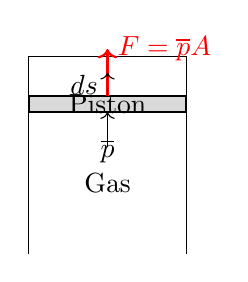
\begin{tikzpicture}
    % Cylinder
    \draw (0,0) -- (0,2.5) -- (2,2.5) -- (2,0);
    % Piston
    \draw[thick, fill=gray!30] (0, 1.8) rectangle (2, 2);
    \node at (1, 1.9) {Piston};
    % Gas pressure
    \node at (1, 0.9) {Gas};
    \node at (1, 1.3) {$\avg{p}$};
    \draw [->] (1, 1.35) -- (1, 1.8); % Arrow indicating pressure
    % Force F=pA
    \draw [->, thick, red] (1, 2) -- (1, 2.6) node[right] {$F=\avg{p}A$};
    % Displacement ds
    \draw [->, dashed] (1, 2.0) -- (1, 2.3) node[midway, left] {$ds$};
\end{tikzpicture}
\end{center}
The mean force on the piston due to the gas pressure is $F = \avg{p}A$.
If the piston moves outward by a small amount $ds$, the work done *by* the gas is:
\[ \ethbar W = F \times ds = (\avg{p}A) ds = \avg{p} (A ds) \]
Since $dV = A ds$ is the change in volume, we have:
\[ \ethbar W = \avg{p} dV \]
Here, the generalized force conjugate to volume $V$ is the mean pressure $\avg{p}$.

If the change in volume $dV$ is quasi-static, then the system is in equilibrium at each volume $V$ during the process, and we can compute the mean pressure $\avg{p}$ at that volume, $\avg{p} = \avg{p}(V)$.
When the system volume changes quasi-statically from $V_i \to V_f$, the total work done is:
\[ W_{if} = \int_{V_i}^{V_f} \ethbar W = \int_{V_i}^{V_f} \avg{p}(V) dV \]

Since $\avg{p} = \avg{p}(V)$, we can graph this relationship in a $p V$-diagram.

\begin{center}
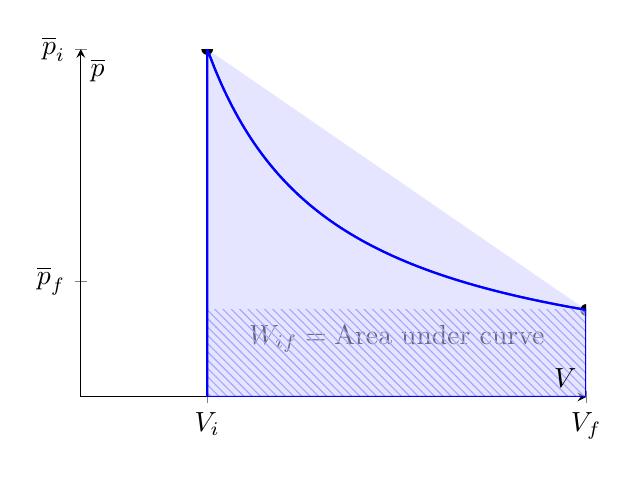
\begin{tikzpicture}
\begin{axis}[
    axis lines=middle, xlabel=$V$, ylabel=$\avg{p}$,
    xmin=0, ymin=0,
    xtick={1, 4}, xticklabels={$V_i$, $V_f$},
    ytick={1, 3}, yticklabels={$\avg{p}_f$, $\avg{p}_i$}, % Adjusted labels
    width=8cm, height=6cm
]
\addplot [domain=1:4, samples=50, smooth, thick, blue, fill=blue!20, fill opacity=0.5] {3/x}; % Example p(V) = const/V
\coordinate (i) at (axis cs:1, 3);
\coordinate (f) at (axis cs:4, 0.75); % Corrected Pf based on 3/V
\node at (i) [circle, fill=black, inner sep=1.5pt, label=above left:i] {};
\node at (f) [circle, fill=black, inner sep=1.5pt, label=below right:f] {};
\node at (axis cs:2.5, 0.5) {$W_{if} = \text{Area under curve}$};
\fill [pattern=north west lines, pattern color=blue!50] (axis cs:1, 0) rectangle (axis cs:4, 0.75);
\addplot [domain=1:4, samples=50, smooth, thick, blue, fill=blue!20, fill opacity=0.5] {3/x} \closedcycle;
\end{axis}
\end{tikzpicture}
\end{center}

Since $\ethbar W = \avg{p} dV$ is an inexact differential, the work $W_{if}$ will, in general, depend on the process (the path taken in the $p V$-diagram).

\begin{center}
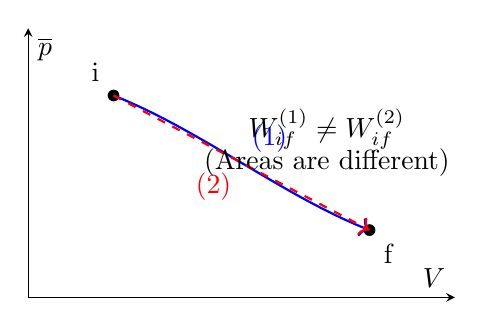
\begin{tikzpicture}
\begin{axis}[
    axis lines=middle, xlabel=$V$, ylabel=$\avg{p}$,
    xmin=0, xmax=5, ymin=0, ymax=4,
    xtick=\empty, ytick=\empty,
    width=7cm, height=5cm
]
\coordinate (i) at (axis cs:1, 3);
\coordinate (f) at (axis cs:4, 1);
\node at (i) [circle, fill=black, inner sep=1.5pt, label=above left:i] {};
\node at (f) [circle, fill=black, inner sep=1.5pt, label=below right:f] {};

% Path 1 (e.g., curve)
\draw [thick, blue, ->] (i) .. controls (2,2.5) and (3,1.5) .. (f) node[midway, above right] {(1)};
% Path 2 (e.g., straight line)
\draw [thick, red, dashed, ->] (i) -- (f) node[midway, below left] {(2)};

\node at (axis cs:3.5, 2.5) {$W_{if}^{(1)} \neq W_{if}^{(2)}$};
\node at (axis cs:3.5, 2.0) {(Areas are different)};
\end{axis}
\end{tikzpicture}
\end{center}

\section*{Approach to Equilibrium}

Return briefly to the notion of "equilibrium".
Recall: For a given macrostate (determined, e.g., by fixed volume $V$ and conserved total energy $E$), there are very many accessible $\mu$-states ($\# = \OmegaE$).
\begin{itemize}
    \item \textbf{Equilibrium:} Probability to find the system in any $\mu$-state, $P(\mu)$, is time-independent ($\implies$ macro parameters are time-independent).
    \item \textbf{Postulate:} An isolated system in equilibrium is equally likely to be in any accessible $\mu$-state.
\end{itemize}
What if a system is *not* equally likely to be in any accessible $\mu$-state?
\begin{itemize}
    \item By the postulate above, this situation cannot be equilibrium.
    \item The system will evolve in time.
\end{itemize}

\textbf{Example:} Gas initially confined to 1/2 of a box by a partition.

\begin{center}
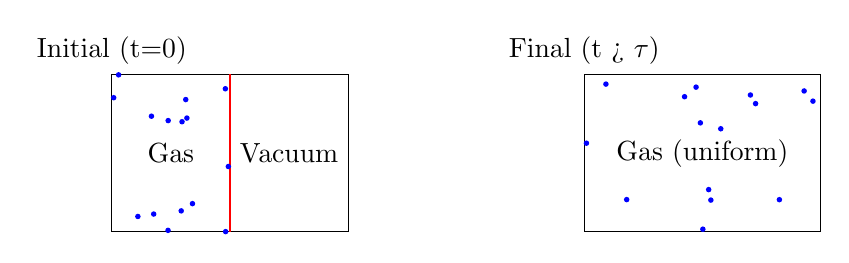
\begin{tikzpicture}
    % Initial State
    \begin{scope}[xshift=-3cm]
        \node at (0, 2.3) {Initial (t=0)};
        \draw (0,0) rectangle (3,2); % Box
        \draw [thick, red] (1.5, 0) -- (1.5, 2); % Partition
        % Gas particles (dots) in left half
        \foreach \i in {1,...,15} {
            \pgfmathsetmacro{\x}{1.5*rnd}
            \pgfmathsetmacro{\y}{2.0*rnd}
            \fill [blue] (\x,\y) circle (1pt);
        }
        \node at (0.75, 1) {Gas};
        \node at (2.25, 1) {Vacuum};
    \end{scope}
    % Final State
    \begin{scope}[xshift=3cm]
        \node at (0, 2.3) {Final (t > $\tau$)};
        \draw (0,0) rectangle (3,2); % Box (no partition)
        % Gas particles spread out
        \foreach \i in {1,...,15} {
            \pgfmathsetmacro{\x}{3.0*rnd}
            \pgfmathsetmacro{\y}{2.0*rnd}
            \fill [blue] (\x,\y) circle (1pt);
        }
         \node at (1.5, 1) {Gas (uniform)};
    \end{scope}
\end{tikzpicture}
\end{center}

Immediately after the partition is removed, the system is not equally likely to be in any accessible state (since 1/2 of the container is empty). This situation will not last long. The system will evolve with time, and after a relatively short time ($\sim \tau$), the density of particles will be uniform over the entire box. The system reaches a new equilibrium state.

\textbf{General Principle:}
\begin{itemize}
    \item If at some time $t$, an isolated system is only in a subset of accessible states, we anticipate a time-evolution toward a distribution in which *all* accessible $\mu$-states are equally likely.
    \item Similarly, if we perturb an equilibrium system and drive it out of equilibrium, we expect the system will eventually return to equilibrium once the perturbation has been "turned off".
    \item Associated with the attainment of equilibrium is a time scale $\tau$, the "relaxation time". The value of $\tau$ varies significantly between different systems.
\end{itemize}
(Proof of statements regarding approach to equilibrium is contained in Boltzmann's H-theorem - see Reif App. A.12).

\end{document}